% Crucial Preamble
\documentclass[12pt,letterpaper]{article} \usepackage{amsmath} \usepackage{graphicx} \usepackage[margin=1in]{geometry} \usepackage{longtable}  \usepackage{amssymb}

% Extra Preamble
\usepackage{fancyhdr} \usepackage{enumitem} \usepackage{float} \usepackage{soul}
\usepackage{multicol} \usepackage[compact]{titlesec}


% frames with display breaks
\usepackage{mdframed}
\allowdisplaybreaks

% change spacing
\usepackage{setspace}
\setlength{\parskip}{0.4\baselineskip}

% Remove paragraph indentation
\setlength{\parindent}{0pt}

% Reduce space before and after section headings
%\titlespacing*{\section}{0pt}{0.1\baselineskip}{0.2\baselineskip}

% changes font
%\renewcommand{\familydefault}{\sfdefault}

% adds header and footer
\pagestyle{fancy}
\fancyhead{} \fancyhead[C]{MAT 2377 Summary Sheet} \fancyhead[L]{MAT2377} \fancyhead[R]{Owen Daigle}
\fancyfoot{} \fancyfoot[C]{\thepage}


\begin{document}
	
	\begin{center}
		\Large\textbf{MAT 2377 Summary Sheet} \\
		\vspace{0.5em}
	\end{center}
	
	\section{Chapter 1: Probabilities}
	%m1 was this chapter
	The \textbf{sample space} is the set of all possible outcomes. 
	
	An \textbf{event} is a collection of outcomes in the sample space. Usually this is what we are looking to work with. 
	
	We can count items using the $k$ stage procedure. 
	
	If we have $k$ stages, each with $n_1$, $n_2$, $n_3$, ... possibilities, then the total number of possiblilites is just $n_1\cdot n_2\cdot n_3\cdot ...\cdot n_k$.
	
	\subsection{Ordered Samples}
	If we have an ordered sample, then we see that picking $1, 2, 3$ is different than picking in a different order $1, 3, 2$.
	
	If we draw r items from a bag of n items:
	\begin{itemize}[]
		\item If we replace each item after drawing, we have: $n\cdot n\cdot n\cdot ... = n^r$ possibilities
		\item If we do NOT replace the items, we have: $n\cdot (n-1)\cdot (n-2)\cdot ...\cdot (n-r) = \frac{n!}{(n-r)!}= {}_nP_r$
	\end{itemize}
	
	\subsection{Unordered Samples}
	This is when the order of the samples does not matter, so $1,2,3$ would be the same as $1,3,2$. 
	
	We can see the number of unordered samples possible with $r$ draws in a sample space of size $n$ using:
	\begin{align*}
		\frac{n!}{(n-r)!r!} = {}_nC_r
	\end{align*}

	\begin{mdframed}
	\textbf{Ex. }20 Items are sampled from a factory. The probability of an item being defective is 0.1. What is the probability of exactly 1 defective item?
	
	To do this, we know that for there to be exactly 1 defective item, there must be 19 working items. 
	
	But there are more than one way that this 1 defective item can be placed. It can be the first item we test, the second item we test, and so on. We do this by $\binom{20}{1}$.
	\begin{align*}
		P(\text{1 Defective Item}) = \binom{20}{1} 0.1^1 (1-0.1)^{19} = 0.27
	\end{align*}
	If we changed this do exactly 2 items, the formula would change to:
	\begin{align*}
		P(\text{2 Defective Items}) = \binom{20}{2} 0.1^2 (1-0.1)^{18} = 0.285
	\end{align*}
	\end{mdframed}
	
	\subsection{Probabilities}
	The probability of an event $A$ with $N$ total outcomes and $a$ favourable outcomes is just:
	\begin{align*}
		P(A) = \frac{a}{N}
	\end{align*}
	
	We can add probabilities using the following formula:
	\begin{align*}
		P(A\cup B) &= P(A) + P(B) - P(A\cap B) \\
		P(A\cup B \cup C) &= P(A)+P(B)+P(C)-P(A\cap B) - P(A\cap C) - P(B\cap C) + P(A\cap B\cap C)
	\end{align*}

	Any 2 events that satisfy the following expression are called \textbf{independant. }
	\begin{align*}
		P(A\cap B) = P(A)\cdot P(B)
	\end{align*}

	\begin{mdframed}
		\textbf{Ex. }The probability of event A is 0.95, and of event B is 0.98. The probability of them both is 0.94. What is the probability of neither of them occurring?
		
		We have:
		\begin{align*}
			P(A)=0.95\qquad P(B)=0.98\qquad P(A\cap B)=0.94
		\end{align*}
		We want:
		\begin{align*}
			P(A\cup B)\prime = 1-P(A\cup B) = 1- (P(A) - P(B) + P(A\cap B)) = 0.01
		\end{align*}
	\end{mdframed}

	\subsection{Conditional Probability}
	We say that the probability of event $B$ given that event $A$ has already happened is:
	\begin{align*}
		P(B|A) = \frac{P(A\cap B)}{P(A)}
	\end{align*}
	
	\subsection{Law of Total Probability}
	This basically works off of the fact that all probabilities must add up to 1. 
	
	This is the specific case to 2 events $A$ and $B$:
	\begin{align*}
		P(B) = P(B|A)P(A) + P(B|\overline A)P(\overline A)
	\end{align*}

	This uses the fact that $A$ and $\overline A$ are mutually exclusive, and exaustive (covers all of $S$). 
	
	So in general, if we have $A_1, A_2, ..., A_k$ and $A_1, A_2, ..., A_k$ are mutually exclusive and exaustive, then we say:
	\begin{align*}
		P(B) = P(B|A_1)P(A_1) + P(B|A_2)P(A_2) + ... + P(B|A_k)P(A_k)
	\end{align*}
	
	\subsection{Bayes Theorum}
	This is a way to get the opposite conditional probability to what we have. 
	
	If we have $P(A|B)$, among a couple other things, we can obtain $P(B|A)$ with:
	\begin{align*}
		P(A|B) = \frac{P(B|A)\cdot P(A)}{P(B)}
	\end{align*}
	
	\begin{mdframed}
		\textbf{Ex. }We have a disease. A test for the disease was given to 450 patients who are known to have this disease. 436 were positive. It was also given to 1000 people without the disease where 10 tests were positive. The known rate of this disease is 15\%. What is the probability of someone having the disease given the test is positive?
		
		I will let $D$ represent Having the Disease, and $P$ represent the Test being Positive.
		
		We have the following information from the question:
		\begin{align*}
			P(P|D) = 436/450 \qquad P(P|D\prime ) = 10/1000 \qquad P(D) = 0.15 \qquad P(D| P) = ?
		\end{align*}
		We can use Bayes theorum to find $P(D|P)$
		\begin{align*}
			P(D|P) = \frac{P(P|D)P(D)}{P(P)}
		\end{align*}
		To find the denominator, we can use the law of total probability. 
		\begin{align*}
			P(P) = P(P|D)P(D) + P(P|D\prime)P(D\prime) = \frac{436}{450}0.15 + \frac{10}{1000}(1-0.15) = 0.1538
		\end{align*}
		And now I can substitute back into Bayes theorum to solve:
		\begin{align*}
			P(D|P) = \frac{P(P|D)P(D)}{P(P)} = \frac{436/450 \cdot 0.15}{0.1538} = 0.945
		\end{align*}
	\end{mdframed}


	
	\section{Chapter 2: Discrete Random Variables}
	%m2 included this chapter
	A random variable is a variable (typically a capital letter) that associates a number to every outcome of an experiment. 
	
	We have 2 functions:
	\begin{itemize}
		\item Probability Distribution Function (PDF) ($f(x)$)
		\item Cumulative Distribution Function (CDF) ($F(x)$)
	\end{itemize}

	The PDF specifies the probability of getting this specific value. 
	
	The CDF specifies the probabilitu of getting anything below this specific value. 
	\begin{center}
		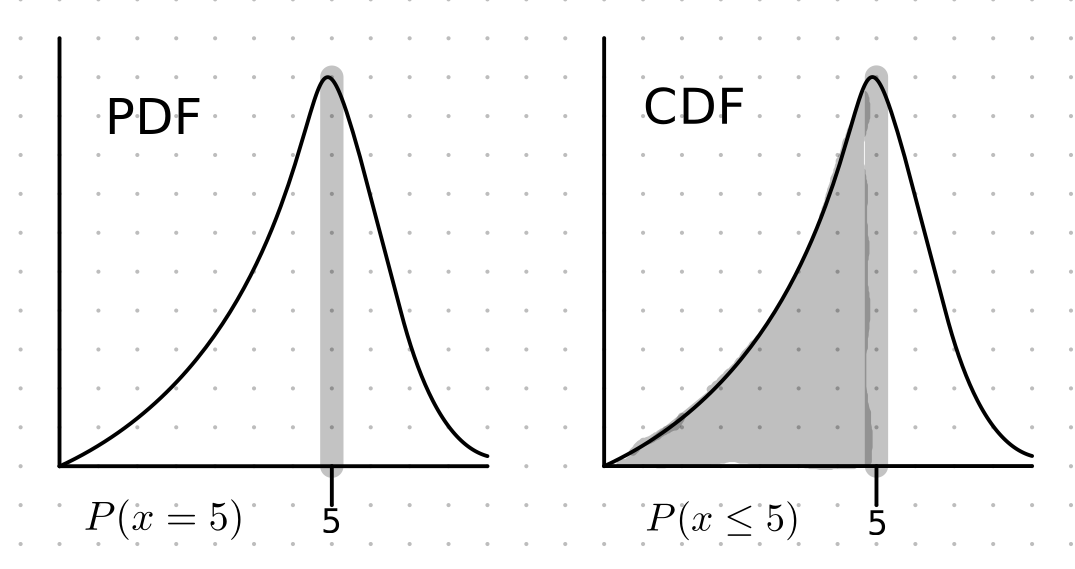
\includegraphics[width=0.7\linewidth]{pdf-vs-cdf}
	\end{center}

	\begin{mdframed}
		\textbf{Ex. } We have a standard fair D6. 
		
		We know that the PDF is $\frac{1}{6}$ for each value. 
		
		The CDF is a bit more complex in that it is $\frac{1}{6}$ for 1, $\frac{2}{6}$ for 2, up to $\frac{6}{6} = 1$ for 6. 
		
		\begin{align*}
			P(X=4) &= \frac{1}{6} &\text{Using PDF}\\
			P(X\le 4) &= \frac{4}{6}  &\text {Using CDF}\\
			P(3\le X\le 5) &= P(X\le 5) - P(X\le 3) = \frac{5}{6} - \frac{3}{6} + \frac {1}{6} &\text{Using CDF}
		\end{align*}
		For the third example, we need to add the extra $\frac{1}{6}$ since we are doing from 3 to 5 inclusively. So 3 or 4 or 5. Taking away $X\le 3$ also takes away 3, so we need to add it back.
	\end{mdframed}
	
	Note that the sum of all PDFs is always 1. The highest CDF is also 1. 
	
	\subsection{Expectation}
	The expectation of a random variable is basically the mean of the variable. We say that this is:
	\begin{align*}
		\mathbb E (u(x)) = \sum u(x)P(X=x)
	\end{align*}

	\begin{mdframed}
		\textbf{Ex. } The expectation of a fair D6 is:
		\begin{align*}
			\mathbb E (X) = \sum xP(X=x) = 1\cdot\frac{1}{6} + 2\cdot \frac{1}{6} + 3\cdot \frac{1}{6} + ... + 6\cdot \frac{1}{6} = 3.5
		\end{align*}
	\end{mdframed}
	
	\subsection{Variance}
	While the mean shows the average of the data, the variance shows how close most of the data is to this average. This can be calculated using the expectation formula:
	\begin{align*}
		\text{Var}(X) = \mathbb E (X^2) - \mathbb E(X)^2
	\end{align*}
	We define the standard deviation as the square root of the variance. 
	\begin{align*}
		\text{SD}(X) = \sqrt{\text{Var}(X)}
	\end{align*}

	\begin{mdframed}
		\textbf{Ex.} Find the variance for the fair D6.
		
		This is very simple, we just use the variance formula. We already have $\mathbb E(X)$, so we can square that for the second term. $\mathbb E(X^2)$ is the more annoying one. 
		\begin{align*}
			\text{Var}(X) &= \mathbb E (X^2) - \mathbb E(X)^2 = \sum x^2 P(X=x) - 3.5^2\\
			&= 1^2 \cdot \frac{1}{6} + 2^2 \cdot \frac{1}{6} + 3^2 \cdot \frac{1}{6} + ... + 6^2 \cdot \frac{1}{6} - 3.5^2 = CALC
		\end{align*}
	If we wanted standard deviation, this would just be square rooting the previous value. 
	\end{mdframed}
	
	\subsection{Binomial Distribution}
	A \textbf{Bernouille Trial} is an expreiment where there are only 2 outcomes: Success, and Failure. We say that $p$ is the probability of success. 
	
	A \textbf{Binomial Experiment} is a series of $n$ bernouille trials.
	
	If we have a random variable $X$ that follows a binomial distribution, then we have the following mean and variance:
	\begin{align*}
		&\mathbb E(X) = np &\text{Var}(X) = np(1-p)
	\end{align*}
	The PDF is:
	\begin{align*}
		P(X=x)= \binom{n}{x}p^x(1-p)^{n-x}
	\end{align*}

	\begin{mdframed}
		\textbf{Ex. }There are 20 samples taken from a process. 1\% of samples have problems. X is the number of samples that have problems. What is the probability that the number of samples exceeds its mean by 3 standard deviations?
		
		So we need to get the mean and standard deviations. These can easily be calculated since this follows a binomial distribution:
		\begin{align*}
			\mathbb E(X) = np = 20\cdot 0.01 = 0.2 \qquad \text{Var}(X) = np(1-p) = 0.2(0.99) = 0.198\\
			\text{SD}(X) = \sqrt{0.198} = 0.44
		\end{align*}
		Now we can find that $P(X>\mathbb E(X) + 3\text{SD}(X)) = P(X > 1.535)$. But since we are working with discrete variable, we can only have integers. $P(X>2) = 1- P(X\le 1)$. We use the complement since it is would be very hard to do 18 calculations. 
		
		Now we need to actually calculate $1-P(X\le 1)$.
		\begin{align*}
			P(X=0) &= \binom{20}{0}0.01^0 0.99^{20} = CALC\\
			P(X=1) &= \binom{20}{1}0.01^1 0.99^{19} = CALC\\
			P(X\le 1) &= 1- P(X=0) - P(X=1) = CALC
		\end{align*}
	\end{mdframed}
	
	\subsection{Geometric Distribution}
	This is a distribution where we want to know the number of steps before the first success occurs. Such as the average number of basketball throws needed to score the first point. 
	
	We have the following mean and variance:
	\begin{align*}
		&\mathbb E(X) = \frac{1}{p} &\text{Var}(X) = \frac{1-p}{p^2}
	\end{align*}
	The PDF is:
	\begin{align*}
		P(X=x)=(1-p)^{x-1}p
	\end{align*}

	The negative binomial distribution is similar except we change it to the number of steps before the \textbf{$r$th} success. 
	\begin{align*}
		&\mathbb E(X) = \frac{r}{p} &\text{Var}(X) = \frac{r(1-p) }{p^2}
	\end{align*}
	The PDF is:
	\begin{align*}
		P(X=x)= \binom{x-1}{r-1} (1-p)^{x-r}p^r
	\end{align*}

	\subsection{Poisson Distribution}
	The poisson distribution works off of a rate. We have the parameter $\lambda$ which is the number of arrivals in a fixed period of time. 
	
	We have the following mean and variance:
	\begin{align*}
		&\mathbb E(X) =\lambda &\text{Var}(X) = \lambda
	\end{align*}

	The PDF is:
	\begin{align*}
		P(X=x) = \frac{\lambda^xe^{-\lambda}}{x!}
	\end{align*}
	
	\section{Chapter 3: Continuous Random Variables}
	%m2 did this chapter
	These are similar to discrete random variables, except for there are infinite number of outcomes. They are in a range, so it is not impossible to work with, but it requires different methods.
	
	For example, the heights of a population are not constrained to certain values such as 100lb, 110lb, 120lb. Someone can be 113.223lb. However, there are upper and lower limits such as potentially 5lb up to 500lb.
	
	If we are given a PDF, we need to integrate over an interval of that PDF in which it basicaly becomes a CDF. 
	
	\subsection{Expectation}
	The expectation can be found by integrating the PDF function between the upper and lower limit of the data. 
	\begin{align*}
		\mathbb E(h(x)) = \int_{-\infty}^{\infty}h(x)f(x)
	\end{align*}

	\begin{mdframed}
		\textbf{Ex. }We are given the following CDF. Find the mean.
		\begin{align*}
			F(x) = \begin{cases}
				0 & \text{if } x \leq 0 \\
				\frac{x}{2} & \text{if } 0 < x < 2 \\
				1 & \text{if } x \geq 2
			\end{cases}
		\end{align*}
	
		To get the mean, we need to integrate the PDF. We are given the CDF. 
		
		We can get the PDF by taking the derivative of the CDF to get:
		\begin{align*}
			f(x) = F\prime (x) = \begin{cases}
				0 & \text{if } x \leq 0 \\
				\frac{1}{2} & \text{if } 0 < x < 2 \\
				1 & \text{if } x \geq 2
			\end{cases}
		\end{align*}
		Then we can integrate this from 0 to 2:
		\begin{align*}
			\mathbb E(x) = \int_0^2 x \cdot \frac{1}{2} = \frac{1}{2}\left[\frac{x^2}{2}\right]^2_0 = 1
		\end{align*}
	\end{mdframed}

	Variance and Standard Deviation are defined in the same way as with discrete variables. 
	
	\subsection{Normal Distribution}
	This is a continuous distribution that has a specific PDF function.
	
	If a variable Z is normally distributed with \textbf{mean of 0} and \textbf{variance of 1}, we say $Z \approx \mathcal{N}(0,1)$.
	
	We represent the normal distribution by Phi ($\Phi$). 
	\begin{align*}
		\Phi(z) = P(Z\le z)
	\end{align*}

	If the mean and variance is not 0 and 1 respectively, we can convert it using the following equation:
	\begin{align*}
		\frac{x-\mu}{\sigma} = Z \approx N(0,1)
	\end{align*}

	We then have a standard normal table found in the appendix. 
	
	\begin{mdframed}
		\textbf{Ex. }If we have a mean of 10s to kill a chicken jockey, and a standard deviation of 10s, what is the probability of taking more than 18.2 seconds to kill that pesky chicken jockey?
		
		Notice that we are given the value in terms of standard deviation $\sigma$ instead of variance $\sigma^2$. 
		
		We will normalize this value and then we can use the normal value to look it up in the normal table (found in the appendix).
		\begin{align*}
			P(X\ge 18.2) &= 1-P(X\le 18.2) = 1-\Phi\left(\frac{18.2-10}{4}\right) = 1-\Phi\left(2.05\right) \\
			&= 1-0.9798=0.0202 \approx 2\%
		\end{align*}
		This value was found on the normal table:
		\begin{center}
			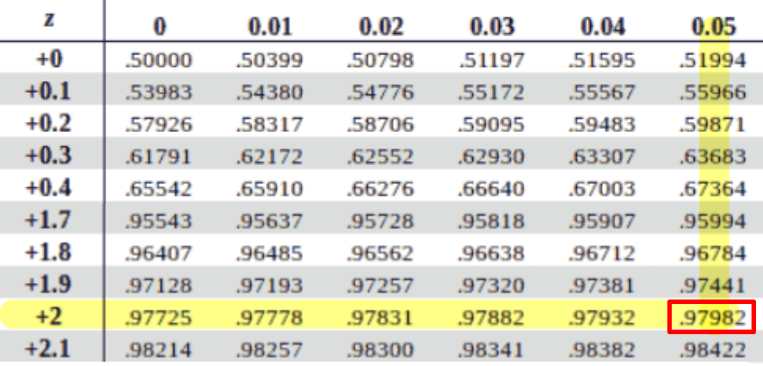
\includegraphics[width=0.5\linewidth]{normal-ex2}
		\end{center}
		
	\end{mdframed}
	
	\begin{mdframed}
		\textbf{Ex. }If we have X normally distributed with mean 10, and variance of 1 ($X\approx \mathcal N(10,1^2)$) then find the value of c such that $P(X\le c) = 0.7019$.
		
		Here we need to do a bit of reverse engineering. We start with finding out what the normal value ($\Phi$) will be to get 0.7019. I look on the normal table and get 0.53.
		\begin{center}
			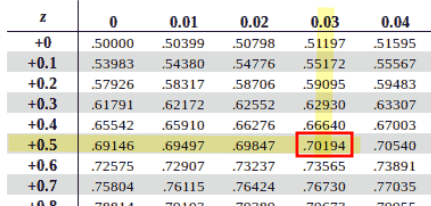
\includegraphics[width=0.5\linewidth]{normal-ex1}
		\end{center}
		Now I know that to get this value of 0.53 I need to apply the normal conversion equation since mean is not 0, and variance is not 1. 
		\begin{align*}
			\frac{x-\mu}{\sigma} = Z \implies \frac{x-10}{\sqrt{1}} = 0.53 \implies x = 10.53
		\end{align*}
		Note that in the normal distribution $\mathcal N(0,1)$, it uses the \textbf{variance} ($\sigma^2$) not standard deviation ($\sigma$). So that is why we square root the 1 on the denominator.
		
	\end{mdframed}
	
	\subsection{Exponential Distribution}
	This distribution is a poisson proccess with rate of $\lambda$. We have:
	\begin{align*}
		f(x) = \lambda e^{-\lambda x}  \qquad \mathbb E(X)=\frac{1}{\lambda} \qquad \text{Var}(X) = \frac{1}{\lambda^2}
	\end{align*}
	
	\subsection{Gamma Distribution}
	This distribution is like the geometric distribution from chapter 2. It is the waiting time for the \textbf{rth arrival}. 
	\begin{align*}
		f(x) = \frac{x^{r-1}}{(r-1)!}\lambda^re^{-\lambda x}  \qquad \mathbb E(X)=\frac{r}{\lambda} \qquad \text{Var}(X) = \frac{r}{\lambda^2}
	\end{align*}
	
	\subsection{Joint Distributions}
	%TODO figure this out
	
	\section{Chapter 4: Descriptive Statistics and Sampling}
	% midterm 3 content
	To describe a dataset, we have measures of central tendancy such as mean and median, and measures of spread such as standard deviation, quartiles, and inter-quartile-range. 
	
	The median is just the middle value of a \textbf{sorted} dataset. If there are 2 middle values, we just take the mean of both of those. 
	
	The mean is just:
	\begin{align*}
		MEAN = \overline{x} = \frac{x_1 + x_2 + ... + x_n}{n}
	\end{align*}

	The median is often used since it is not heavily influenced by outliers unlike mean. 
	
	\subsection{Quartiles}
	The quartile is like taking the median of the lower half of the data (under the true median). 
	\begin{center}
		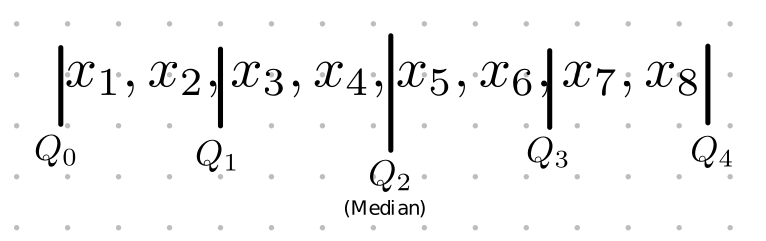
\includegraphics[width=0.4\linewidth]{quartiles}
	\end{center}
	We call the \textbf{Inter Quartile Range (IQR)} as the difference between the third and first quartile $IQR = Q_3-Q_1$

	We identify a datapoint $x$ as an \textbf{outlier} if:
	\begin{align*}
		x < Q_1 - 1.5IQR \qquad \text{or} \qquad x>Q_3 + 1.5IQR
	\end{align*}

	\subsection{Sample Statistics}
	If we do not know the variance of a whole dataset (such as the entire earths population) then we can consider a sample of this population to estimate the population. 
	
	We have \textbf{sample standard deviation $s$} and \textbf{sample variance $s^2$}. These estimage the standard deviation $\sigma$ and variance $\sigma^2$ respectively. 
	\begin{align*}
		s^2 = \frac{1}{n-1}\sum^{n}_{i=1}(x_i - \overline x)^2
	\end{align*}

	\subsection{Skewness}
	We call a dataset \textbf{left skewed} of the tail of the data is to the left (outliers on the left) or \textbf{right skewed} if the tail of the data is on the right (outliers on the right).
	\begin{center}
		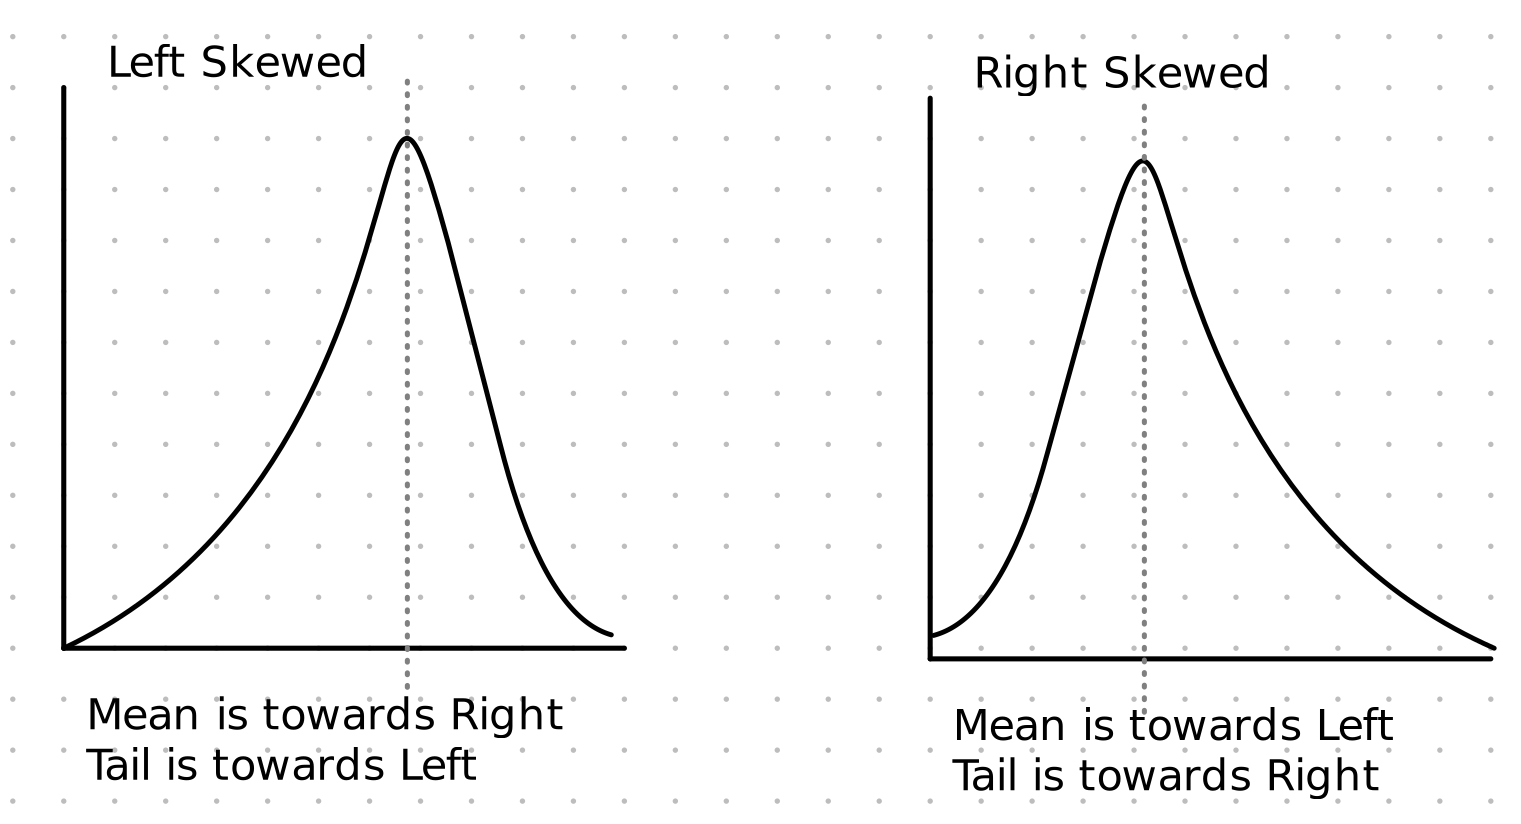
\includegraphics[width=0.6\linewidth]{skew}
	\end{center}

	\subsection{Independant and Identically Distributed (IID) Case}
	When all variables are independant and identically distributed we say the expected value and variance of the entire set is just the number of variables times the variance/expected value of one item.
	\begin{align*}
		\mathbb E\left[\sum_{i=1}^{n}X_i\right]=n\mu \qquad \text{Var}\left[\sum_{i=1}^{n}X_i\right]=n\sigma^2
	\end{align*}
	Then we say that if we are considering a sample of these, we have:
	\begin{align*}
		\mathbb E [\overline X] = \mu \qquad \text{Var} [\overline X] = \frac{\sigma^2}{n}
	\end{align*}
	We can also use the normal distribution if the population is normally distributed to model $\sum_{i=1}^n X_i$ or $\overline X$.
	
	\subsection{Central Limit Theorum}
	This states that as the \textbf{number of runs of an experiment increases}, it will start to reach a \textbf{normal distribution}. This is regardless of whether or not the individual experiments are normal or not. 
	
	\subsection{Difference between 2 Means}
	We can work with 2 variables $X_1, X_2, ..., X_n$ with $\mu_1, \sigma^2_1$, and $Y_1, Y_2, ..., Y_m$ with $\mu_2, \sigma_2^2$ using the following formula:
	\begin{align*}
		Z = \frac{\overline X - \overline Y - (\mu_1 - \mu_2)}{\sqrt{\frac{\sigma_1^2}{n}+\frac{\sigma^2_2}{m}}}
	\end{align*}

	\subsection{Other Distributions}
	We have 2 other main distributions. The \textbf{Chi squared} ($\chi^2$) distribution, and \textbf{Student's t} distribution. 
	
	Student's t distribution is used when the population variance is unknown, and we have to approximate using the sample variance (standard deviation). This is found in the appendix.
	
	Both of these distributions have the \textbf{degrees of freedom} ($v$ or $df$) which is usually just $n-1$. This happens since we take away one degree of freedom by estimating the variance. 
	
	\section{Chapter 5: Point and Interval Estimation} 
	% midterm 3 content
	This chapter is mostly about confidence intervals (CI). 
	
	We have 2 main confidence intervals that we use. Each of them has an \textbf{$\alpha$ value} where if we say the $n$ percent interval, we have $\alpha = 1-n$.
	
	So for the 95\% confidence interval, $\alpha = 0.05$. 
	
	The 2 main confidence intervals are the \textbf{95 percent, and 99 percent}. 
	
	\subsection{CI When $\sigma$ is known}
	We can use a \textbf{normal distribution} to model this since we know $\sigma$, $n$, and $\overline X$. 
	
	We use the equation:
	\begin{align*}
		CI = \overline X \pm Z_{\alpha/2} \frac{\sigma}{\sqrt n}
	\end{align*}

	Using the normal table we can get $Z_{\alpha/2}$. For $\alpha = 0.05$ we have $Z_{0.025} = 1.96$ and for $\alpha = 0.01$ we have $Z_{0.005} = 2.575$.
	
	\subsection{CI When $\sigma$ is unknown}
	Here we have to find the sample variance $s$ and we know $n$, and $\overline X$.
	
	We use \textbf{Student's t distribution} with the equation:
	\begin{align*}
		CI = \overline X \pm t_{\alpha/2}(n-1) \frac{s}{\sqrt n}
	\end{align*}
	Recall that $n-1$ is the degrees of freedom for the t distribution.
	
	\subsection{CI For a Proportion}
	When we are dealing with a proportion for a binomial distributions (2 options, either success of failure), we say that $P$ is the probability of success. 
	
	We can model this using the \textbf{normal distribution} using:
	\begin{align*}
		CI = P \pm z_{\alpha/2} \sqrt{\frac{P(1-P)}{n}}
	\end{align*}

	\section{Chapter 6: Hypothesis Testing}
	This chapter is about hypotheses. We create 2 hypotheses. The first one, $H_1$ is the alternative hypothesis. We test it against the null hypothesis $H_0$. We do the test for $H_0$ and we either \textbf{reject} the null hypothesis in favour of $H_1$, or \textbf{fail to reject} the null hypothesis. We reject the null if evidence against the null is \textbf{strong}.
	
	\subsection{Types of Errors}
	
	We commit a \textbf{Type 1 error} if we reject $H_0$ when $H_0$ is actually true. The probability of a type 1 error is:
	\begin{align*}
		\alpha = P(\text{reject }H_0 | H_0\text{ is True})
	\end{align*}
	
	We commit a \textbf{Type 2 error} if we fail to reject $H_0$ when $H_0$ is actually false. The probability of a type 2 error is:
	\begin{align*}
		\beta= P(\text{fail to reject }H_0| H_0 \text{ is False})
	\end{align*}
	
	\subsection{Types of Hypotheses}
	Typically we are testing if the mean is the same as we expect (null), or if it differs (alternative).
	
	We say that:
	\begin{align*}
		H_0&: \mu = \mu_0 &\text{Null Hypothesis}\\
		H_1&: \mu \ne \mu_0 &\text{Two Sided Alternative}\\ 
		&\text{ OR } \mu<\mu_0 &\text{Left Sided Alternative}\\
		&\text{ OR } \mu>\mu_0 &\text{Right Sided Alternative}
	\end{align*}
	
	\subsection{Test for Mean with Known Variance}
	If the population is normal, or it has a \textbf{large number of samples} ($n$ is large), then we can use a \textbf{normal distribution} to approximate the test. 
	
	We can get a value from the normal distribution using the variance, mean, and number of samples. 
	
	\subsection{Test for Mean with Unknown Variance}
	If we do not know the variance, we can use \textbf{Student's t distribution.}
	
	\subsection{Two Sample Test}
	%TODO figure this out
	
	\section{Chapter 7: Linear Regresion}
	
	\subsection{Correlation Coefficient}
	The \textbf{coefficient of correlation} $\rho$ between 2 variables $x$ and $y$ is:
	\begin{align*}
		\rho_{xy} = \frac{\sum (x_i-\overline x)(y_i-\overline y)}{\sqrt{\sum (x_i - \overline x)^2 \sum(y_i - \overline y)^2}} = \frac{S_{xy}}{\sqrt{S_{xx}S_{yy}}}
	\end{align*}
	We can also wright these as:
	\begin{align*}
		S_{xy} &= \sum x_iy_i - n\overline x \overline y\\
		S_{xx} &= \sum x_i^2 - n\overline x ^2\\
		S_{yy} &= \sum y_i^2 - n\overline y ^2
	\end{align*}
	
	\subsection{Linear Regression}
	We can get a line of best fit using the equation of:
	\begin{align*}
		Y = \beta_0 + \beta_1 X+ \epsilon
	\end{align*}
	Here $\epsilon$ is the error term which is often omitted. 
	
	The $\beta_1$ can be found using the following equation:
	\begin{align*}
		\beta_1 = \frac{S_{xy}}{S_{xx}}
	\end{align*}
	The $\beta_0$ can be found by subbing in a known values for the equation of $\overline y = \beta_0 + \beta_1 \overline x$ and solving for $\beta_0$.
	
	We can also estimate the \textbf{variance} by doing:
	\begin{align*}
		\hat \sigma^2 = \frac{S_{yy} - \beta_1 S_{xy}}{n-2w}
	\end{align*}
	
	\subsection{Hypothesis Testing}
	We can do hypothesis testing using these $\beta$ values such as where:
	\begin{align*}
		H_0: \beta_0 = \beta_{0,0} \qquad H_1: \beta_0 \ne \beta_{0,0}
	\end{align*}
	Similarly to chapter 6, this result is often \textbf{normally distributed} so can be easily calculated using the normal table. 
	
	\newpage
	\section{Appendix}
	\subsection {Normal Distribution Table (Z-Table)}
	\begin{center}
		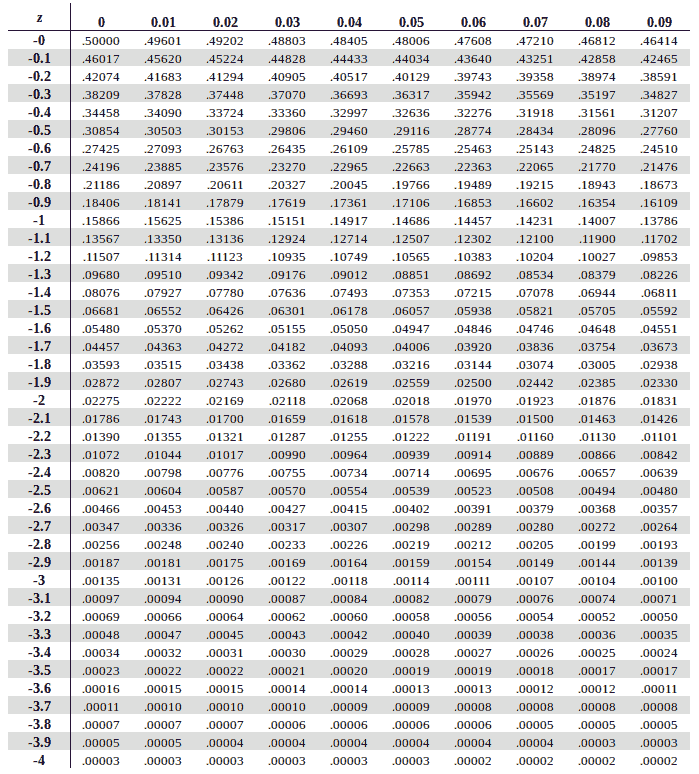
\includegraphics[width=0.99\linewidth]{negativeztable}
	\end{center}
	\begin{center}
		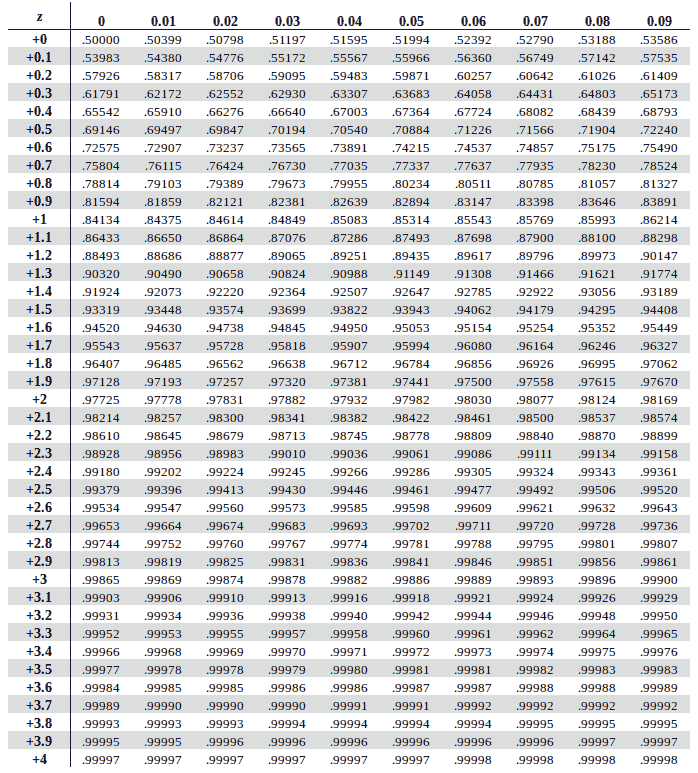
\includegraphics[width=0.99\linewidth]{positiveztable}
	\end{center}
	Tables taken from https://www.ztable.net/
	
	\subsection{Student's t Table}
	\begin{center}
		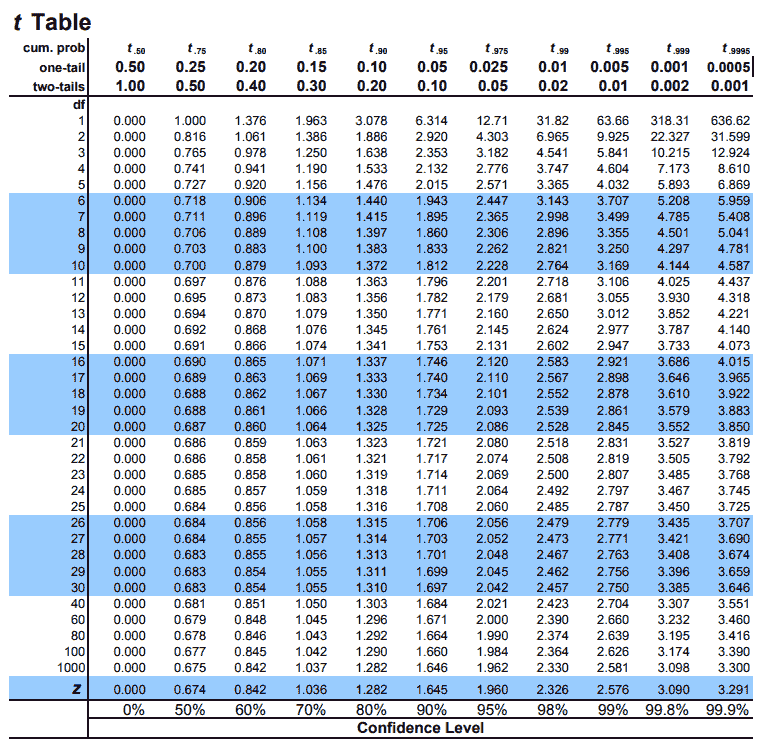
\includegraphics[width=0.99\linewidth]{t-table}
	\end{center}
	Table taken from https://www.tdistributiontable.com/
	
	
\end{document}